% ---------------------------------------------------------------------------
\FloatBarrier
\section{Unseen Batch and Interpretation (RQ5)}
\label{sec:unseen}

The secondary test set is one new batch. This phase asks how the models
transfer to a second one: the 2018-02-20 batch (\texttt{u1},
Sections~\ref{sec:dataset}--\ref{sec:eda}), which is not part
of~\cite{severson2019} and was not used for any choice so far. It has 39
labelled cells, 30 standard and 9 \texttt{-newstructure}. No model was refitted
or re-tuned: every model of Phases~2--4 was fitted on the 41 training cells
with its earlier settings and applied once to \texttt{u1}
(\texttt{src/p5\_unseen.py}). Models are then explained with SHAP values
(\texttt{src/p5\_shap.py}); \texttt{notebooks/05\_unseen\_batch.ipynb} shows
every step. Because \texttt{u1} is not in the paper, there are no published
numbers to compare with.

\subsection{What is different about this batch}
Before the lives were used, the inputs of \texttt{u1} were compared with the
training cells. The standard cells rest about 10\,min per cycle and hold 3.6\,V
for about 20\,min (cycles of 70\,min, Table~\ref{tab:steps}); the
\texttt{-newstructure} cells use 5-second rests, as in the secondary batch. Half of
the standard cells and two thirds of the \texttt{-newstructure} cells use a
policy that also appears in training. Several features lie far outside the
training range (median $z$-scores against the training cells): for the
standard cells the temperature integral ($+2.9$), the capacity at cycle 2
($+2.6$) and the overhang rise ($+2.6$); for the \texttt{-newstructure} cells
$\log_{10}\mathrm{Var}(\dq)$ ($-1.5$) and the minimum IR ($-2.6$). For about a
third of the cells the temperature integral or the overhang rise is more
than three standard deviations from the training mean, so the models
extrapolate in their inputs, although the lives (392--1186 cycles) lie inside
the training range. Six cells have no IR record; their IR features are set to
the training median.

\subsection{Pre-registered hypotheses}
Five hypotheses, each with a decision rule, were fixed in the code before any
\texttt{u1} life was used. The main models are the elastic net on F2, F3 and
F4 and the GP on F4.
\begin{itemize}
  \item[H1] The models separate the two groups but rank cells poorly within a
  group. Rule: for at least three main models, Spearman $\rho\ge0.7$ over all
  cells and $<0.5$ within each group.
  \item[H2] The late overhang rise of the standard cells makes $\dq$
  understate their degradation. Rule: the elastic net on F2 over-predicts the
  standard cells, its residual increases with \texttt{overhang\_after10} within
  them, and the F4 models are less biased.
  \item[H3] The \texttt{-newstructure} cells, with the procedure of the
  secondary batch, are mispredicted in the same direction as that batch.
  Rule: same sign of the mean signed error for at least three main models.
  \item[H4] The full model's temperature integral lowers the predictions for
  the standard cells. Rule: mean SHAP contribution below $-0.05$ in
  $\log_{10}$ life.
  \item[H5] The GP on F4 is overconfident. Rule: its 95\,\% interval covers
  fewer than 90\,\% of the cells.
\end{itemize}

\subsection{Results}
Table~\ref{tab:p5res} and Fig.~\ref{fig:p5parity} give the results.

\begin{table*}[t]
\centering
\caption{Frozen models on the unseen batch: RMSE (cycles) / mean
percentage error / mean signed percentage error (bias; positive =
over-prediction). Upper block: the pre-registered main models and the
baselines; lower block: the other models of Phases~2--4.}
\label{tab:p5res}
\small
\begin{tabular}{@{}lccc@{}}
\toprule
Model & All 39 cells & Standard (30) & \texttt{-newstructure} (9) \\
\midrule
Constant (training geometric mean) & 226 / 36.8\,\% / $+22$\,\% & 173 / 38.2\,\% / $+38$\,\% & 351 / 32.4\,\% / $-32$\,\% \\
Policy mean & 236 / 34.6\,\% / $+18$\,\% & 168 / 34.3\,\% / $+34$\,\% & 384 / 35.6\,\% / $-36$\,\% \\
Elastic net, F2 (discharge) & 260 / 27.1\,\% / $+27$\,\% & 104 / 20.4\,\% / $+20$\,\% & 506 / 49.5\,\% / $+50$\,\% \\
Elastic net, F3 (full) & 138 / 12.8\,\% / $+12$\,\% & 51 / 9.2\,\% / $+9$\,\% & 271 / 24.6\,\% / $+23$\,\% \\
Elastic net, F4 & 178 / 20.4\,\% / $-2$\,\% & 97 / 17.6\,\% / $-11$\,\% & 325 / 30.0\,\% / $+30$\,\% \\
GP, F4 & 158 / 13.9\,\% / $+9$\,\% & 49 / 9.1\,\% / $+2$\,\% & 316 / 30.1\,\% / $+30$\,\% \\
\midrule
Elastic net, F1 (variance) & \textbf{119} / 15.2\,\% / $+11$\,\% & 77 / 14.3\,\% / $+10$\,\% & \textbf{204} / 18.5\,\% / $+17$\,\% \\
Elastic net, F3 + F4 & 124 / \textbf{9.2\,\%} / $+6$\,\% & \textbf{28} / \textbf{5.0\,\%} / $0$\,\% & 254 / 23.0\,\% / $+23$\,\% \\
GP, F2 & 237 / 26.0\,\% / $+26$\,\% & 102 / 20.5\,\% / $+20$\,\% & 458 / 44.4\,\% / $+44$\,\% \\
SVR, F2 / F4 & 242 / 587 & 144 / 624 & 430 / 440 \\
Additive splines, F2 / F4 & 346 / 553 & 183 / 545 & 639 / 579 \\
PLS, curve / F4 + shape & 5371 / 298 & 416 / 106 & 11155 / 591 \\
\bottomrule
\end{tabular}
\end{table*}

\begin{figure*}[t]
  \centering
  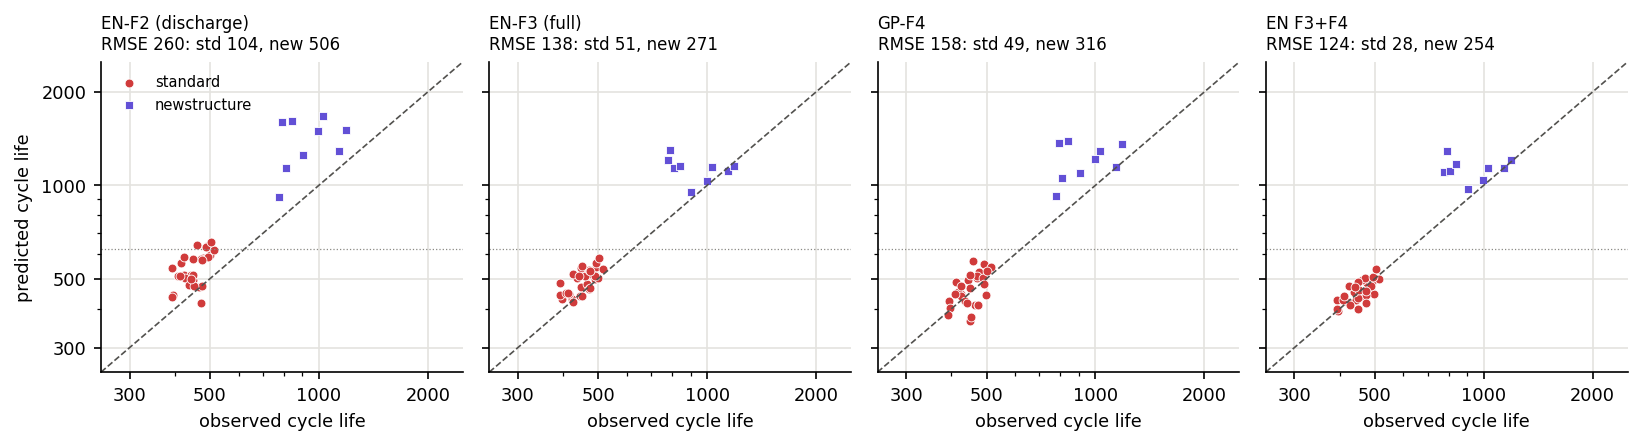
\includegraphics[width=\textwidth]{fig_p5_parity}
  \caption{Predicted vs.\ observed cycle life on the unseen batch for four
  frozen models. Dotted: training geometric mean (constant baseline).}
  \label{fig:p5parity}
\end{figure*}

\textbf{The standard cells transfer well.} The elastic net on F3 and the GP
on F4 predict them to within about 50 cycles (9\,\%), and the elastic net on
F3 + F4 to within 28 cycles (5\,\%), better than on the paper's own primary
test set. These cells resemble the 2017-06-30 training batch in their rests
and lives. Within this group, the paper's models also rank the cells
reasonably ($\rho=0.58$ for F2, $0.64$ for F3).

\textbf{The \texttt{-newstructure} cells are over-predicted by every model,
by 17--50\,\%.} Their $\dq$ is small, which the models read as a long life
(most predictions between 1000 and 1700 cycles), but they live 777--1186 cycles. The
secondary batch, with the same 5-second rests, showed a bias of only
$\pm3$--5\,\%.

\textbf{The model ranking differs from the secondary set.} The paper's
discharge model, the best on the secondary set, is the worst main model here
and worse than the constant baseline overall (260 vs.\ 226 cycles), while the
full model, the worst on the secondary set, does well. The simplest model,
$\log_{10}\mathrm{Var}(\dq)$ alone, has the lowest RMSE overall (119 cycles) and the
smallest bias on the \texttt{-newstructure} cells ($+17\,\%$): with fewer
features there is less to extrapolate. A paired bootstrap
(5000 resamples) resolves the main differences: over all cells, F4 beats F2 by
80 cycles (95\,\% interval 37--121) and F3 beats F2 by 121 (44--189) with the
elastic net, and the GP on F4 beats the elastic net on F4 by 21 (7--38); on the
standard cells the GP on F4 beats the elastic net on F4 by 48 (30--66).

\textbf{Flexible models fail when their inputs leave the training range.}
SVR and the additive splines on F4 over-predict by about 70\,\%, because the
overhang rise of many \texttt{u1} cells lies far beyond the training range;
PLS on the whole curve fails as on the secondary set.

\textbf{Uncertainty.} The 95\,\% intervals of the GP on F4 cover 87\,\% of the
cells: 97\,\% of the standard cells but only 56\,\% of the \texttt{-newstructure}
cells. The intervals are honest where the model is right and overconfident
where it is wrong.

\begin{table}[t]
\centering
\caption{Verdicts of the pre-registered hypotheses.}
\label{tab:p5hyp}
\setlength{\tabcolsep}{3pt}
\begin{tabular}{@{}lcp{0.66\columnwidth}@{}}
\toprule
& Verdict & Evidence \\
\midrule
H1 & no & standard cells ranked better than expected ($\rho$ 0.58, 0.64 for F2, F3); only the GP on F4 met the rule \\
H2 & no & F2 over-predicts the standard cells ($+20\,\%$) and the F4 models are less biased, but within the standard cells the residual \emph{decreases} with the overhang rise ($\rho=-0.43$) \\
H3 & yes (weak) & same sign for 3 of 4 models, but $+23$ to $+50\,\%$ here against $\pm3$--5\,\% on the secondary set \\
H4 & yes & temperature integral lowers the standard cells by $-0.089$ in $\log_{10}$ life ($\approx-19\,\%$) \\
H5 & yes & GP-F4 coverage 87\,\% (standard 97\,\%, \texttt{-newstructure} 56\,\%) \\
\bottomrule
\end{tabular}
\end{table}

Table~\ref{tab:p5hyp} summarises the verdicts. The failure of H2 matters for
Section~\ref{sec:physics}: the explanation given there for the overhang
feature (lithium released inside the $\dq$ window hides degradation) fits the
group-level pattern but not the cell-level test, so it remains a hypothesis.

\subsection{Interpretation with SHAP}
For the main models and the elastic net on F3 + F4, exact SHAP values of the
predicted $\log_{10}$ life were computed with the training cells as
background. Because $\log_{10}|\min\dq|$ and $\log_{10}\mathrm{Var}(\dq)$ are almost
collinear, their individual values are read together.

\begin{table}[t]
\centering
\caption{Share of mean $|\mathrm{SHAP}|$ per feature on the training cells
and on the unseen batch (\%). F4: GP; F3, F3 + F4: elastic net.}
\label{tab:p5imp}
\setlength{\tabcolsep}{3pt}
\begin{tabular}{@{}lcccccc@{}}
\toprule
& \multicolumn{2}{c}{F3} & \multicolumn{2}{c}{F4 (GP)} & \multicolumn{2}{c}{F3 + F4} \\
Feature & train & u1 & train & u1 & train & u1 \\
\midrule
$\dq$ (min + variance) & 42 & 33 & -- & -- & 26 & 21 \\
\texttt{margin\_rate} & -- & -- & 74 & 64 & 20 & 13 \\
\texttt{overhang\_after10} & -- & -- & 26 & 36 & 4 & 8 \\
Temperature integral & 18 & 31 & -- & -- & 18 & 32 \\
Charge time & 16 & 6 & -- & -- & 14 & 5 \\
Capacity at cycle 2 & 12 & 23 & -- & -- & 8 & 16 \\
Minimum IR & 11 & 8 & -- & -- & 9 & 6 \\
\bottomrule
\end{tabular}
\end{table}

Table~\ref{tab:p5imp} shows that $\dq$ information, directly or through
\texttt{margin\_rate}, is the largest driver in every model; in the paper's
discharge model $\dq$ minimum and variance carry 64\,\% of the attribution on
the training cells. About a third of the full model rests on the temperature
integral and the charge time. On \texttt{u1} the attribution moves towards the
features that lie outside the training range there (temperature integral,
capacity at cycle 2, overhang rise): the models lean most on what they know
least.

Fig.~\ref{fig:p5shap} decomposes the mean prediction of each test set into
feature contributions and compares it with the actual mean. It explains the
behaviour on \texttt{u1}:
\begin{itemize}
  \item \textbf{F2 over-predicts the standard cells because of their capacity.}
  $\dq$ lowers the prediction ($-0.10$), but the high initial capacity raises
  it ($+0.04$ from the capacity features), giving $-0.06$ against an actual
  $-0.14$. This, not the overhang, is the source of the bias tested in H2.
  \item \textbf{F3 is right on the standard cells partly for the wrong reason.}
  The temperature integral, in effect the long cycle duration, lowers the
  prediction by 0.09 and cancels the capacity effect.
  \item \textbf{The GP on F4 beats the elastic net on F4 because it learned
  that the overhang effect saturates.} Fig.~\ref{fig:p5overhang} shows the SHAP
  value of \texttt{overhang\_after10}: the elastic net extrapolates it as a
  straight line, down to $-0.38$ for a 10.8\,mAh rise, and under-predicts the
  standard cells by 11\,\%; the GP's effect flattens beyond about 2\,mAh inside the
  training range and falls more gently outside it, which gives the right
  answer ($+2\,\%$). The flattening was learned from the training cells alone.
  \item \textbf{The \texttt{-newstructure} over-prediction comes from $\dq$
  itself.} All four models attribute $+0.27$ to $+0.34$ to the $\dq$ features,
  against an actual $+0.18$: these cells change their discharge curve less than
  cells of the same life in the training and secondary batches. No single
  out-of-range feature is responsible; why the relation differs for this group
  is an open question.
\end{itemize}

\begin{figure*}[t]
  \centering
  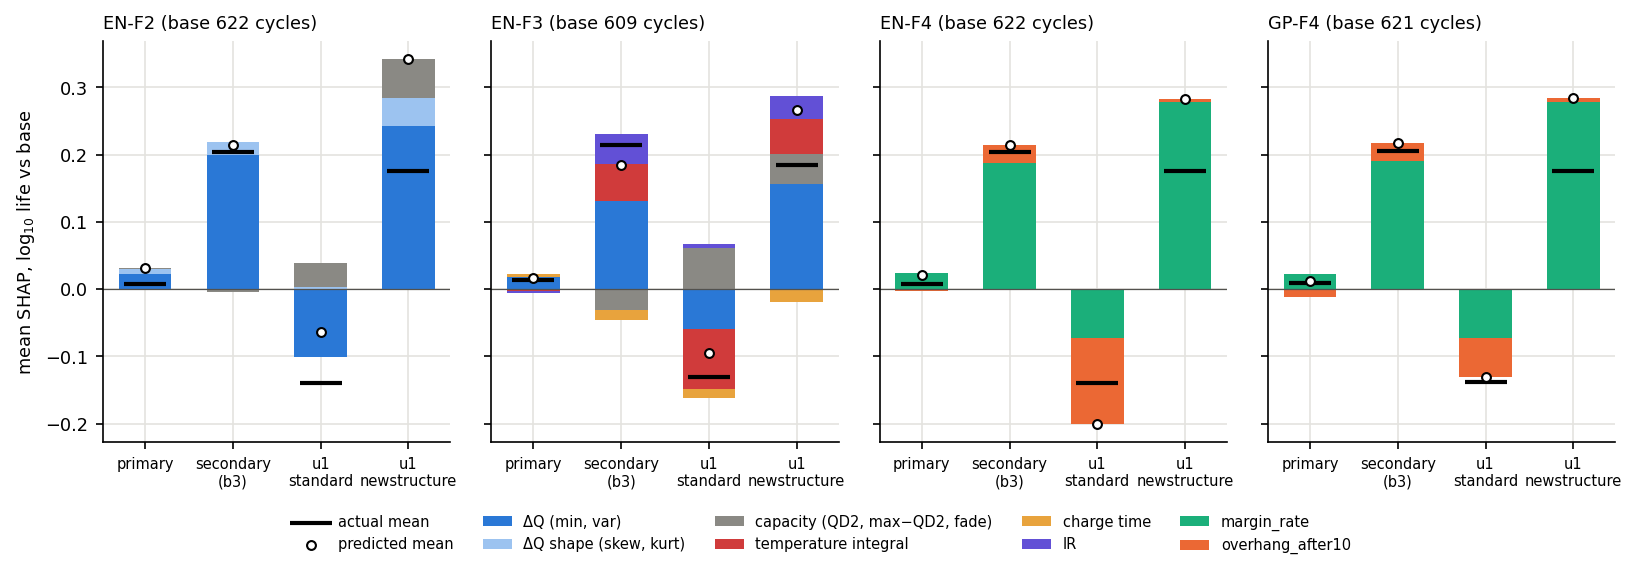
\includegraphics[width=\textwidth]{fig_p5_shap}
  \caption{Mean SHAP contributions per test set (bars, grouped features),
  mean prediction (open circle) and actual mean (black line), in $\log_{10}$
  life relative to the model's mean training prediction. The gap between
  circle and line is the bias.}
  \label{fig:p5shap}
\end{figure*}

\begin{figure}[t]
  \centering
  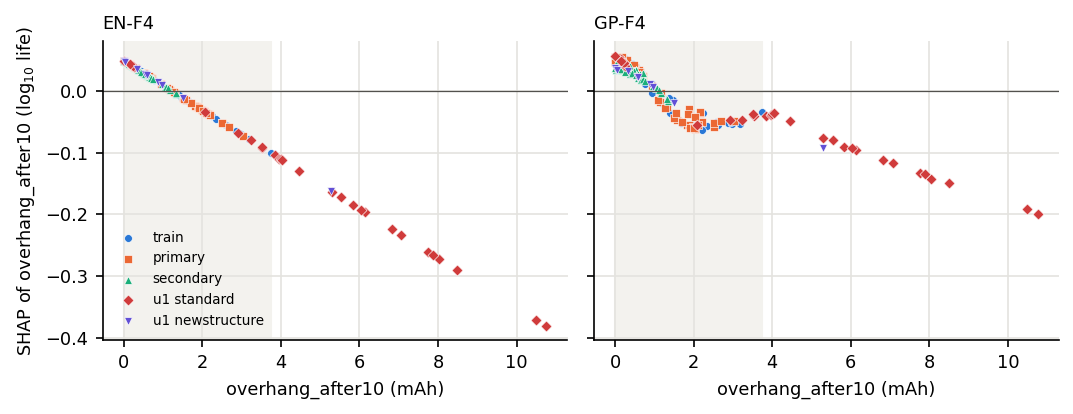
\includegraphics[width=\columnwidth]{fig_p5_overhang}
  \caption{SHAP value of \texttt{overhang\_after10} against its value, for
  the elastic net and the GP on F4. Shaded: range of the training cells.}
  \label{fig:p5overhang}
\end{figure}

\subsection{Exploratory check: GP on F3 + F4}
After all test sets had been used, the GP was also fitted to the eleven
features of F3 + F4. This configuration was not pre-registered, so its scores
are an after-the-fact check. It nearly memorises the training cells (training
RMSE 19 cycles), has the worst nested cross-validation error of the compared
models (0.0626 against 0.0478 for the GP on F4), and its fitted kernel gives short
length-scales to seven features, including the temperature integral and the
charge time. On the test sets it is no better than the elastic net on the same
features (primary 112 vs.\ 122, secondary 210 vs.\ 205, \texttt{u1} 129 vs.\ 124
cycles) and worse than the GP on F4 on the paper's sets. The GP works best with
few, robust features.

\subsection{Answer to RQ5}
Transfer to a new batch depends on how its procedure relates to the training
batches. For the standard cells of the unseen batch, which resemble a training
batch, several models predict to within 5--10\,\%. For the
\texttt{-newstructure} cells every model over-predicts by 17--50\,\%, because their
discharge curve changes less than their life implies. Which model transfers
best differs between the two new batches: the paper's discharge model is the
best on the secondary set and the worst on this one, and the full model the
reverse. Features that encode the batch help when the new batch resembles a
training batch and hurt when it does not; flexible models fail when their
inputs leave the training range. The GP on F4 is the most balanced choice:
close to the best on all three test sets, with uncertainty that is honest for
cells like those in training.

\textbf{Caveats.} The unseen batch has only nine \texttt{-newstructure}
cells. Many models were evaluated on it (Table~\ref{tab:p5res}); the
pre-registered main comparisons and the bootstrap intervals should be relied
on, not the best of all rows. The elastic net on F3 + F4 performs best overall
but was not a pre-registered main model.
